\documentclass[15pt]{beamer}
\usepackage{graphicx}
\graphicspath{ {./assets/graph.png} }
%~~~~~~~~~~~~~~~~~~~~~~~~~~~~~~~~~~~~~~~~~~~~~~~~~~~~~~~~~~~~~~~~~~~~~~~~~~~~~~
% Use roboto Font (recommended)
\usepackage[sfdefault]{roboto}
\usepackage[utf8]{inputenc}
\usepackage[T1]{fontenc}
%~~~~~~~~~~~~~~~~~~~~~~~~~~~~~~~~~~~~~~~~~~~~~~~~~~~~~~~~~~~~~~~~~~~~~~~~~~~~~~

%~~~~~~~~~~~~~~~~~~~~~~~~~~~~~~~~~~~~~~~~~~~~~~~~~~~~~~~~~~~~~~~~~~~~~~~~~~~~~~
% Define where theme files are located. ('/styles')
\usepackage{styles/fluxmacros}
\usefolder{styles}
% Use Flux theme v0.1 beta
% Available style: asphalt, blue, red, green, gray 
\usetheme[style=asphalt]{flux}
%~~~~~~~~~~~~~~~~~~~~~~~~~~~~~~~~~~~~~~~~~~~~~~~~~~~~~~~~~~~~~~~~~~~~~~~~~~~~~~

%~~~~~~~~~~~~~~~~~~~~~~~~~~~~~~~~~~~~~~~~~~~~~~~~~~~~~~~~~~~~~~~~~~~~~~~~~~~~~~
% Extra packages for the demo:
\usepackage{booktabs}
\usepackage{colortbl}
\usepackage{ragged2e}
\usepackage{schemabloc}
%~~~~~~~~~~~~~~~~~~~~~~~~~~~~~~~~~~~~~~~~~~~~~~~~~~~~~~~~~~~~~~~~~~~~~~~~~~~~~~

%~~~~~~~~~~~~~~~~~~~~~~~~~~~~~~~~~~~~~~~~~~~~~~~~~~~~~~~~~~~~~~~~~~~~~~~~~~~~~~
% Informations
\title{\hspace{2pt} EE2227-CONTROL SYSTEMS}
%\subtitle{Modern theme v0.1}
\author{Tejaswini}
\institute{EE18BTECH11047}
\date{\today}
%~~~~~~~~~~~~~~~~~~~~~~~~~~~~~~~~~~~~~~~~~~~~~~~~~~~~~~~~~~~~~~~~~~~~~~~~~~~~~~

\begin{document}

% Generate title page
\titlepage


\begin{frame}{QUESTION}{EE 2017(SET-2)}
	\justifying  \textbf{QUESTION-41} \newline Consider the system described by the following state space representation 
	\newline \newline \begin{bmatrix}\dot x_{1}(t)\\\dot x_{2}(t)
	\end{bmatrix} = \begin{bmatrix}0 & 1 \\ 0 & -2\end{bmatrix}\begin{bmatrix}x_{1}(t)\\x_{2}(t)\end{bmatrix} + \begin{bmatrix}0 \\ 1\end{bmatrix}u(t) \newline \newline \newline
	y(t) = \begin{bmatrix}1 & 0\end{bmatrix}\begin{bmatrix}x_{1}(t)\\x_{2}(t)\end{bmatrix}
	\newline \newline If u(t) is a unit step input and \begin{bmatrix}x_{1}(0) \\ x_{2}(0)\end{bmatrix} = \begin{bmatrix}1 \\ 0 \end{bmatrix} , the value of output y(t) at t = 1 sec(rounded off to three decimal places) is __________
\end{frame}

\def\beamer@mytheme@style{green}
\begin{frame}[fragile]{SOLUTION}
		$\dot X(t)$ = AX(t) + Bu(t)\hspace{70pt}------(1)
		\newline \newline Laplace transform on equation (1) results in 
		\newline \newline sX(s) - x(0) \hspace{5pt}= \hspace{5pt}AX(s) + Bu(s)
		\newline \newline (sI - A)X(s) \hspace{5pt}= \hspace{5pt}x(0) +B$\frac{1}{s}$
		\newline \newline X(s)\hspace{5pt} = \hspace{5pt}(sI - A)^{-1}[x(0) + B\frac{1}{s}]\hspace{55pt}--(2)
		
\end{frame}

\subsection{fonts}

\subsection{footnotes}

\begin{frame}{SOLUTION}
        Y(t)=CX(t)+Du(t)
        \newline\newline Y(t)=CX(t)\hspace{70pt}[Given: D = 0]
	    \newline\newline Y(s) = CX(s)
	    \newline\newline Y(s) = C(sI - A)^{-1}[x(0) + B\frac{1}{s}]\hspace{55pt}--(3)
	    \newline\newline Given ,\newline 
	\newline \hspace{10pt}A = \begin{bmatrix}0 & 1\\0 & -2\end{bmatrix}\hspace{5pt}B = \begin{bmatrix}0\\1\end{bmatrix}\hspace{5pt}C=\begin{bmatrix}1 & 0 \end{bmatrix}
\end{frame}

\section{Collections}
\subsection{lists}

\begin{frame}{SOLUTION}
   sI - A \hspace{5pt}=\hspace{5pt} \begin{bmatrix}s & -1 \\ 0 & s+2\end{bmatrix}\hspace{70pt} \begin{bmatrix}x_{1}(0)\\x_{2}(0)\end{bmatrix} = \begin{bmatrix}1\\0\end{bmatrix}
   \newline \newline\newline (sI - A)^{-1} \hspace{5pt}=\hspace{5pt}\begin{bmatrix}\frac{1}{s} & \frac{1}{s(s+2)}\\0&\frac{1}{s+2}\end{bmatrix}
   \newline\newline  
 \newline Y(s) = \begin{bmatrix}1 & 0 \end{bmatrix}\begin{bmatrix}\frac{1}{s} & \frac{1}{s(s+2)} \\ 0 & \frac{1}{s+2}\end{bmatrix}\begin{bmatrix}\begin{bmatrix}1 \\ 0\end{bmatrix} + \frac{1}{s}\begin{bmatrix}0 \\ 1\end{bmatrix}\end{bmatrix} 
\end{frame}

\subsection{tables}

\begin{frame}{SOLUTION}
Y(s)\hspace{15pt}=\hspace{15pt}\begin{bmatrix}1 & 0 \end{bmatrix}\begin{bmatrix}\frac{1}{s} & \frac{1}{s(s+2)} \\ 0 & \frac{1}{s+2}\end{bmatrix}\begin{bmatrix}1 \\ \frac{1}{s}\end{bmatrix}
\newline \newline \newline Y(s) \hspace{15pt}= \hspace{15pt}\begin{bmatrix}1 & 0 \end{bmatrix}\begin{bmatrix}\frac{1}{s} + \frac{1}{s^{2}(s+2)} \\ \frac{1}{s(s+2)}\end{bmatrix}
\newline\newline\newline Y(s)\hspace{15pt}=\hspace{15pt} $\frac{1}{s} + \frac{1}{s^{2}(s+2)}$
\newline \newline Y(s)\hspace{15pt}=\hspace{15pt}$\frac{1}{4(s+2)}+ \frac{3}{4s} + \frac{1}{2s^{2}}$
\end{frame}

\subsection{blocs}

\begin{frame}[fragile]{SOLUTION}
  	Inverse laplace transform on Y(s) .....
  	\newline \newline y(t) = $(\frac{1}{4}e^{-2t}$ + $\frac{3}{4}$ + $\frac{1}{2}t)u(t)$
  \newline \newline y(1) = $\frac{1}{4}e^{-2}$ + $\frac{3}{4}$ + $\frac{1}{2}(1)$
  \newline \newline y(1) = 1.28383
  \newline \newline Rounding off to three decimals......
  \newline \newline y(1) = 1.284
  	
\end{frame}

\begin{frame}{PLOT}
    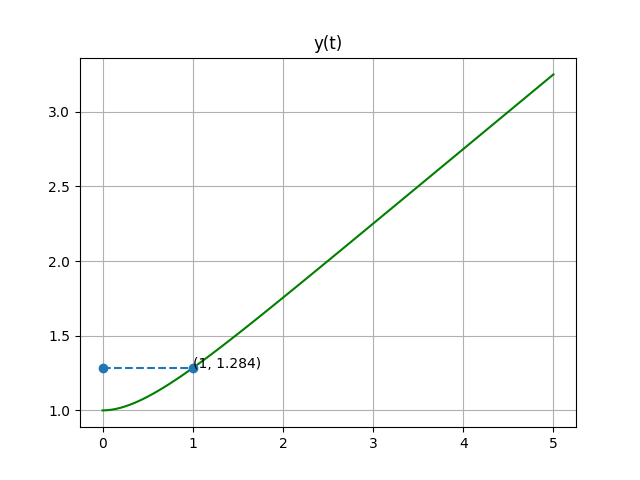
\includegraphics[width = 10cm,height=8.0cm]{assets/graph.png}
\end{frame}
